\documentclass[a4paper]{article}

\usepackage[italian]{babel}
\usepackage[utf8]{inputenc}
\usepackage[T1]{fontenc}
\usepackage{enumitem}
\usepackage{graphicx}
\usepackage{float}
\usepackage{longtable}
\usepackage[table]{xcolor}
\usepackage{geometry}

\usepackage{lastpage}
\usepackage[bottom]{footmisc}
\usepackage{fancyhdr}
\usepackage{tabu}

\usepackage{pgffor}
\usepackage{etoolbox}
\usepackage{multirow}



\usepackage[official]{eurosym}

% Navigazione pdf
\usepackage{hyperref}
\hypersetup{
	colorlinks=true,
	linkcolor=black,
	filecolor=magenta,      
	urlcolor=blue,
}

\usepackage{tabularx}

\usepackage{multicol}
\newcommand{\glo}{\textsubscript{\emph{G}}}
\newcommand\hd{\emph{HD Viz}}
\newcommand\cod{\emph{Code of Duty}}
\newcommand{\myparagraph}[1]{\paragraph{#1}\mbox{}\\}
\newcommand{\mysubparagraph}[1]{\subparagraph{#1}\mbox{}\\}

\newcommand{\NdP}{\emph{Norme di Progetto 3.0.0}}
\newcommand{\PdP}{\emph{Piano di Progetto 3.0.0}}
\newcommand{\AdR}{\emph{Analisi dei requisiti 3.0.0}}
\newcommand{\PdQ}{\emph{Piano di Qualifica 3.0.0}}

\definecolor{header}{HTML}{FA8D21}
\definecolor{pari}{HTML}{DBDBDB}
\definecolor{dispari}{HTML}{F5F5F5}

\setcounter{secnumdepth}{4}

\pagestyle{fancy}
\lhead{
\includegraphics[scale=0.06]{../_template/images/logo_crop.png}}

%Titolo del documento
\rhead{\titolodocumento{}}
\cfoot{Pagina \thepage\ di \pageref{LastPage}}
\renewcommand{\footrulewidth}{0.4pt}

\newcommand{\titolodocumento}{Analisi dei requisiti} % Titolo documento
\newcommand{\versione}{ 2.3.0 } % Versione documento
\newcommand{\approvazione}{ Diego Piola } % Responsabile di progetto
\newcommand{\redazione}{\parbox[t]{4cm} {Andrea Mascari\\Damiano Zanardo\\Diego Piola\\}} % Redattori di questo documento
\newcommand{\verifica}{\parbox[t]{4cm} {Andrea Mascari\\Damiano Zanardo \\ Diego Piola \\ Alessandro Flori \\ } } % Verificatori di questo documento
\newcommand{\stato}{In lavorazione} % Approvato 
\newcommand{\uso}{Esterno} % Interno - Esterno
\newcommand{\destinazione}{\parbox[t]{4cm}{Prof Tullio Vardanega \\ Prof. Riccardo Cardin} } % Destinatario ( D1\\D2\\D3 )
\newcommand{\descrizionedocumento}{Il documento elenca casi d'uso e requisiti del progetto } % Descrizione documento

% Mettere sempre la virgola dopo l'ultima riga, se no si rompe la tabella

\def\modifiche{
    {v0.0.1, 02/12/2020, Damiano Zanardo, Analista , Prima bozza{,} aggiunti tutti i capitolati},
}



% Per modificare il frontespizio e diario delle modifiche andare sulla cartella source
% Per aggiungere il contenuto andare sulla cartella source/sections e creare un nuovo file.tex per ogni sezione

% Per parole che devono andare nel glossario aggiungere /glo{} dopo la parola

\begin{document}
    % Frontespizio 
    %\documentclass[a4paper]{article}
%\usepackage[italian]{babel}
\usepackage[utf8]{inputenc}
\usepackage[T1]{fontenc}
\usepackage{enumitem}
\usepackage{graphicx}
\usepackage{float}
\usepackage{longtable}
\usepackage[table]{xcolor}
\usepackage{geometry}

\usepackage{lastpage}
\usepackage[bottom]{footmisc}
\usepackage{fancyhdr}
\usepackage{tabu}

\usepackage{pgffor}
\usepackage{etoolbox}
\usepackage{multirow}



\usepackage[official]{eurosym}

% Navigazione pdf
\usepackage{hyperref}
\hypersetup{
	colorlinks=true,
	linkcolor=black,
	filecolor=magenta,      
	urlcolor=blue,
}

\usepackage{tabularx}

\usepackage{multicol}
%\begin{document}

\begin{titlepage}

	\begin{center}
		
\includegraphics[scale = 0.5]{../_template/images/logo.png}\\
		\large \textbf{Code of Duty - Progetto \emph{HD VIZ}} \\
		\vfill
		\huge \textbf{\titolodocumento}
		\vspace*{\fill}
        
        \vfill
        \large
    \end{center}
    
	\begin{table}[htbp]
        \centering
        \begin{tabular}{r|l}
            \textbf{Versione} & \versione{} \\
            \textbf{Approvazione} & \approvazione{} \\
            \textbf{Redazione} & \redazione{} \\
            \textbf{Verifica} & \verifica{} \\
            \textbf{Stato} & \stato{} \\
            \textbf{Uso} & \uso{} \\
            \textbf{Destinato a} & \destinazione{}
        \end{tabular}
    \end{table}
    
    \begin{center}
        \vfill
        \normalsize
        \textbf{Descrizione}\\
		\descrizionedocumento
        \vfill
        \small
        \texttt{info@codeofduty.it}
	\end{center}
\end{titlepage}

%\end{document}

    
    % Diario delle modifiche
    \newcommand*\mytablecontents{}
\foreach \x [count=\nj] in \modifiche
{
    \foreach \y [count=\ni] in \x
    {
        \ifnum\ni=6
            \xappto\mytablecontents{\y}
            \gappto\mytablecontents{\\}
            \gappto\mytablecontents{\hline}
        \else
            \xappto\mytablecontents{\y&}
        \fi
    }
}

\section*{Diario delle modifiche}

% Impostazioni della tabella
\tabulinesep = 2mm % padding
\taburowcolors [1] 2{pari .. dispari} % colori delle righe
\begin{longtabu} to \textwidth {| X[0.3, c m] | X[0.6,c m] | X[0.7,c m] | X[0.9,c m] | X[0.7,c m] | X[1.2,l m]|} % larghezza delle colonne
\hline
\rowcolor{header} % colore dell'header

\textbf{Ver.} & \textbf{Data} & \textbf{Nominativo} & \textbf{Ruolo} & \textbf{Verificatore} & \multicolumn{1}{c|}{\textbf{Descrizione}}\\
\hline
\mytablecontents

\end{longtabu}

    \pagebreak
    
    % Indice
    \tableofcontents
    \pagebreak
    
    % Se necessari
    % \listoffigures
    % \listoftables
    
    % Contenuto
    \section{Introduzione}
\subsection{Scopo del documento}
	In questo documento vengono illustrate le modalità con cui il gruppo \textit{Code of Duty} affronterà lo sviluppo del progetto \hd, quali:
	\begin{itemize}
    		\item Analisi dei rischi;
    		\item Presentazione del modello di sviluppo adottato;
    		\item Pianificazione delle attività e divisione dei ruoli;
    		\item Stima dei costi economici e risorse necessarie al compimento del progetto.
	\end{itemize}
\subsection{Scopo del prodotto}
	L'obiettivo del progetto è quello di creare un'applicazione di visualizzazione di dati con molte dimensioni. L'applicazione dovra permettere diverse visualizzazioni dei dati tramite browser ed è richiesta anche una parte server di supporto che permetta il prelevamento dei dati e la loro elaborazione.
\subsection{Glossario}
	In questo documento vengono definiti e descritti tutti i termini e tecnologie al fine di evitare ambiguità relative al linguaggio utilizzato nei documenti formali. Per facilitare la lettura i termini saranno contrassegnati da una 'G' a pedice.  
\subsection{Riferimenti}
	\subsubsection{Normativi}
		\begin{itemize}
			\item \textbf{Norme di Progetto}: \textit{Norme di progetto 2.0.0};
			\item \textbf{Regolamento organigramma e specifica tecnico-economica} : \href{https://www.math.unipd.it/~tullio/IS-1/2020/Progetto/RO.html}{RO}.
		\end{itemize}
	\subsubsection{Informativi}
		\begin{itemize}
			\item \textbf{Capitolato d'interesse}: \href{https://www.math.unipd.it/~tullio/IS-1/2020/Progetto/C4.pdf}{HD Viz - Visualizzazione di dati con molte dimensioni};
			\item \textbf{Il ciclo di vita del Software}: \href{https://www.math.unipd.it/~tullio/IS-1/2020/Dispense/L05.pdf}{L05};
			\item \textbf{Gestione di progetto}: \href{https://www.math.unipd.it/~tullio/IS-1/2020/Dispense/L06.pdf}{L06}.
		\end{itemize}
\subsection{Scadenze}
	Il gruppo \textit{Code of Duty} ha deciso di impegnarsi a rispettare le seguenti scadenze per lo sviluppo del progetto \hd
	\begin{itemize}
		\item \textbf{Revisione dei Requisiti}: 11-Gennaio-2021;
		\item \textbf{Revisione di Progettazione}: 10-Marzo-2021;
		\item \textbf{Revisione di Qualifica}: 2-Aprile-2021;
		\item \textbf{Revisione di Accettazione}: 3-Maggio-2021;
	\end{itemize}

    \pagebreak
    
    \section{Setup}
    \subsection{Requisiti hardware}
    HD Viz richiede le seguenti specifiche hardware:
    \begin{itemize}
        \item \textbf{Processore}: Dual Core;
        \item \textbf{Memoria}: 2GB.
    \end{itemize}
    \subsection{Requisiti software}
        \subsubsection{Requisiti per l'installazione}
        \begin{itemize}
            \item \href{https://yarnpkg.com/}{Yarn v1.22.0} o superiore.
        \end{itemize}
        Se si vuole eseguire il server:
        \begin{itemize}
            \item \href{https://nodejs.org/en/}{Node v14.0.0} o superiore.
        \end{itemize}
    \subsection{Installazione}
    La repository si trova al seguente link:
    \url{https://github.com/CodeOfDutyJS/hdviz}
    \\
    per clonare la repository con Git spostarsi nella cartella dove si desidera mettere il progetto ed eseguire:
    \begin{verbatim}
        git clone https://github.com/CodeOfDutyJS/hdviz
    \end{verbatim}
    alternativamente è possibile scaricare il codice direttamente da Github.
        \subsubsection{Parte Server}
        per eseguire la parte server aprire il terminale e spostarsi nella cartella server con il comando:
        \begin{verbatim}
        cd path/della/cartella/server
        \end{verbatim}
        a questo punto basta eseguire il comando:
        \begin{verbatim}
        node index.js
        \end{verbatim}
        \subsubsection{Parte Client}
        Se si desidera eseguire solo la parte client spostarsi nella cartella client con il comando:
        \begin{verbatim}
        cd path/della/cartella/client
        \end{verbatim}
        a questo punto è necessario installare le dipendenze con il comando: 
        \begin{verbatim}
        yarn
        \end{verbatim}
        o alternativamente con:
        \begin{verbatim}
        yarn install
        \end{verbatim}
        a questo punto si può eseguire un Development Server con il comando:
        \begin{verbatim}
        yarn start
        \end{verbatim}
        la Web App sarà disponibile su localhost alla porta mostrata dal terminale (usualmente la porta 3000). A questo punto basta aprire uno dei browser supportati e immettere l'indirizzo:
        \begin{verbatim}
        http://localhost:3000/
        \end{verbatim}
        nel caso la porta mostrata dal terminale sia diversa dalla porta 3000 sostituire 3000 con la nuova porta nell'indirizzo.
    \pagebreak
    
    \section{Tecnologie}
    \subsection{Tecnologie per lo sviluppo}
    \subsubsection{Javascript}
        Il linguaggio principale usato per l'implementazione di HD Viz è javascript, in particolare viene usata la versione ES2018.
    \subsubsection{ESlint}
        ESlint è uno strumento per l'analisi statica del codice javascript. La configurazione può essere consultata nel file .eslintrc.js. Lo stile di codifica adottato è quello di Airbnb.
    \subsubsection{Parte server}
    In questa sezione vengono elencate le tecnologie utilizzate per la parte server.
        \myparagraph{Node.Js}
        Node.Js è un ambiente runtime di Javascript basato sul motore \href{https://v8.dev/}{V8 Javascript engine}. Node.Js permette d'implementare il cosiddetto paradigma "JavaScript everywhere", difatti sia la parte client che la parte server sono scritte utilizzando questo linguaggio.
        \myparagraph{ExpressJs}
        Express.js è un framework back end che semplifica la creazione di API rest.
        \url{http://expressjs.com/}
    \subsubsection{Parte client}
        \myparagraph{D3.js}
        D3.js è una libreria che permette di manipolare il DOM con un approccio data-driven, in \textit{HD Viz} viene usata principalmente per creare le visualizzazioni.
        \url{https://d3js.org/}
        \myparagraph{React}
        React è un framework JavaScript per la creazione di interfacce utente. Molto flessibile nello sviluppo di web app a singola pagina e mobile. React si occupa del rendering di elementi sul DOM tramite un Virtual DOM che aggiornerà  solamente le componenti che hanno subito un cambiamento. Solitamente viene affiancato da altre librerie per gestire lo state dell'applicazione.
        \myparagraph{Ant Design}
        Ant Design è un framework che utilizzato assieme a React permette la creazione di interfacce utente semplici ed espressive.
    \subsubsection{Testing}
        \myparagraph{Jest}
        Jest è un framework per il testing di codice Javascript, il quale permette di ottenere importanti informazioni dall'esecuzione dei test (code coverage). Fornisce inoltre semplici strumenti per il mock di oggetti esterni.
    \subsubsection{Altre librerie impiegate}
        \myparagraph{ml.js}
        Collezione di librerie JavaScript comprendente vari strumenti utili per applicazioni di Machine Learning. In HD Viz è stata utilizzata per calcolare matrici e distanze tra punti dimensionali.
        \myparagraph{PapaParse}
        Libreria per il parsing di file CSV in oggetti JSON. Viene utilizzata per convertire un file CSV in un formato utile per l'analisi dei dati e con la stessa struttura dei dati che vengono forniti dai database attraverso il server.
    \pagebreak
    
    \section{Architettura del prodotto}

\subsection{Descrizione generale}
In fase di progettazione è stato deciso di dividere il sistema \hd\ in due parti distinte: una web app e un server che riesca a recuperare i dati da diversi tipi di database.

La web app è in grado di recuperare i dati a partire da file csv o di collegarsi al server e recuperare i dati dal database. Sarà possibile scegliere diversi tipi di visualizzazioni e diverse opzioni per creare la visualizzazione più utile per l'analisi dei dati.

La parte server gestisce le chiamate API. Il suo scopo è di fare da interfaccia tra il client e il database a cui esso vuole collegarsi. Essendo possibile collegarsi a diversi tipi di database il server è in grado di gestire e uniformare le risposte delle query sia per database SQL che non.

\subsection{Architettura web app}
    \subsubsection{Descrizione}
    Per sviluppare la web app è stato deciso di utilizzare il pattern architetturale MVVM. Le principali motivazioni dietro questa scelta sono: 
    \begin{itemize}
        \item la web app è stata realizzata tramite React\glo\ e il pattern MVVM è sembrato abbastanza semplice da integrare;
        \item permette di utilizzare i modelli e gli Store in altri contesti senza doverli modificare;
        \item permette di disaccoppiare la parte di \emph{presentation logic} e \emph{business logic}.
    \end{itemize}
    
    Il passaggio dei dati dai Model alle varie View avviene tramite l'utilizzo degli Store (\emph{Model View}). Grazie al \emph{Context} di React\glo\ nelle View è possibile eseguire un binding tra le proprietà dei componenti React\glo\ e gli attributi esposti dagli Store, inoltre è possibile eseguire un binding tra le funzioni dei componenti React\glo\ e i metodi esposti dagli Store.
    
    L'aggiornamento dei dati e le notifiche dei cambiamenti a questi dati avviene grazie all'uso di \emph{MobX}, una libreria per l'implementazione del pattern \emph{Observer} non disponibile nativamente in React\glo .
    
    Per la selezione di una visualizzazione e le operazioni che devono essere eseguite viene utilizzato il pattern \emph{Template Method}.
    Quando un utente seleziona una visualizzazione:
    \begin{itemize}
        \item viene inizializzato il corretto modello di visualizzazione tramite l'oggetto di tipo VisualizationType contenuto all'interno del VisualizationManager.
        \item vengono visualizzate le opzioni relative alla giusta visualizzazione scelta.
    \end{itemize}
    
    \pagebreak
    
    \subsubsection{Diagramma dei package}
    Segue il diagramma dei package della web app.
    
    \begin{figure}[htbp]
        \centering
        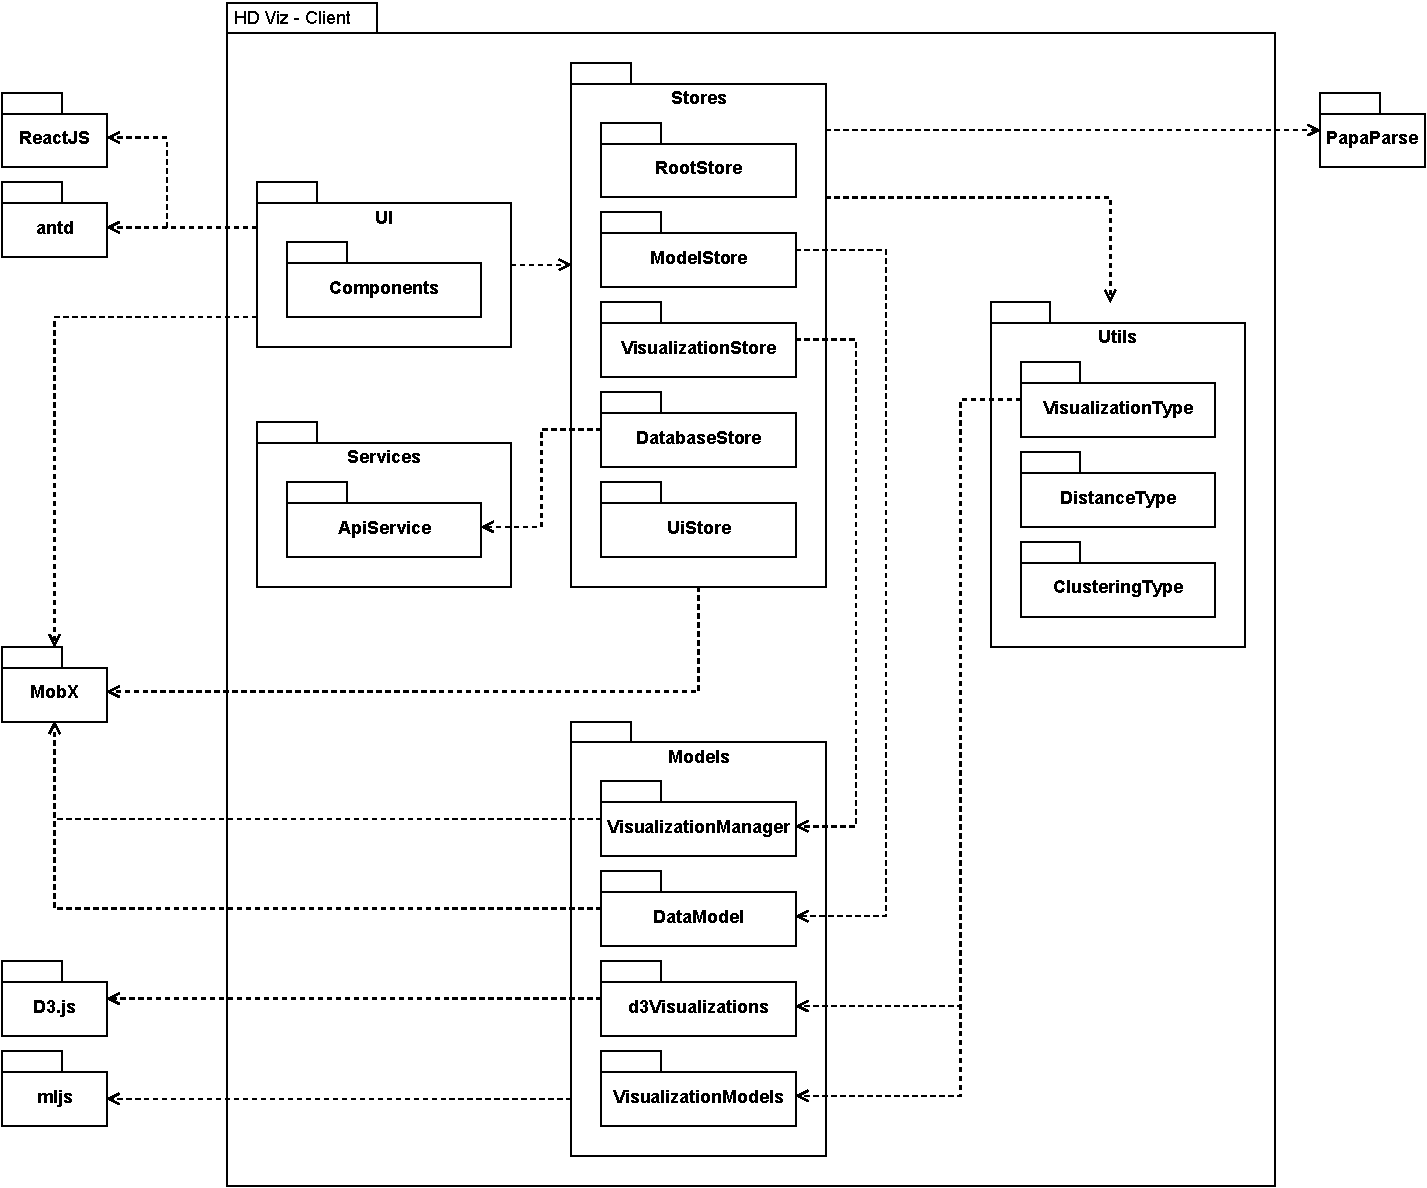
\includegraphics[width=1\textwidth]{source/img/package.pdf}
        \caption{Diagramma dei package della web app}
    \end{figure}
    
    \pagebreak
    
    \subsubsection{Diagrammi delle classi}
    Segue il diagramma delle classi della web app.
    \begin{figure}[H]
        \centering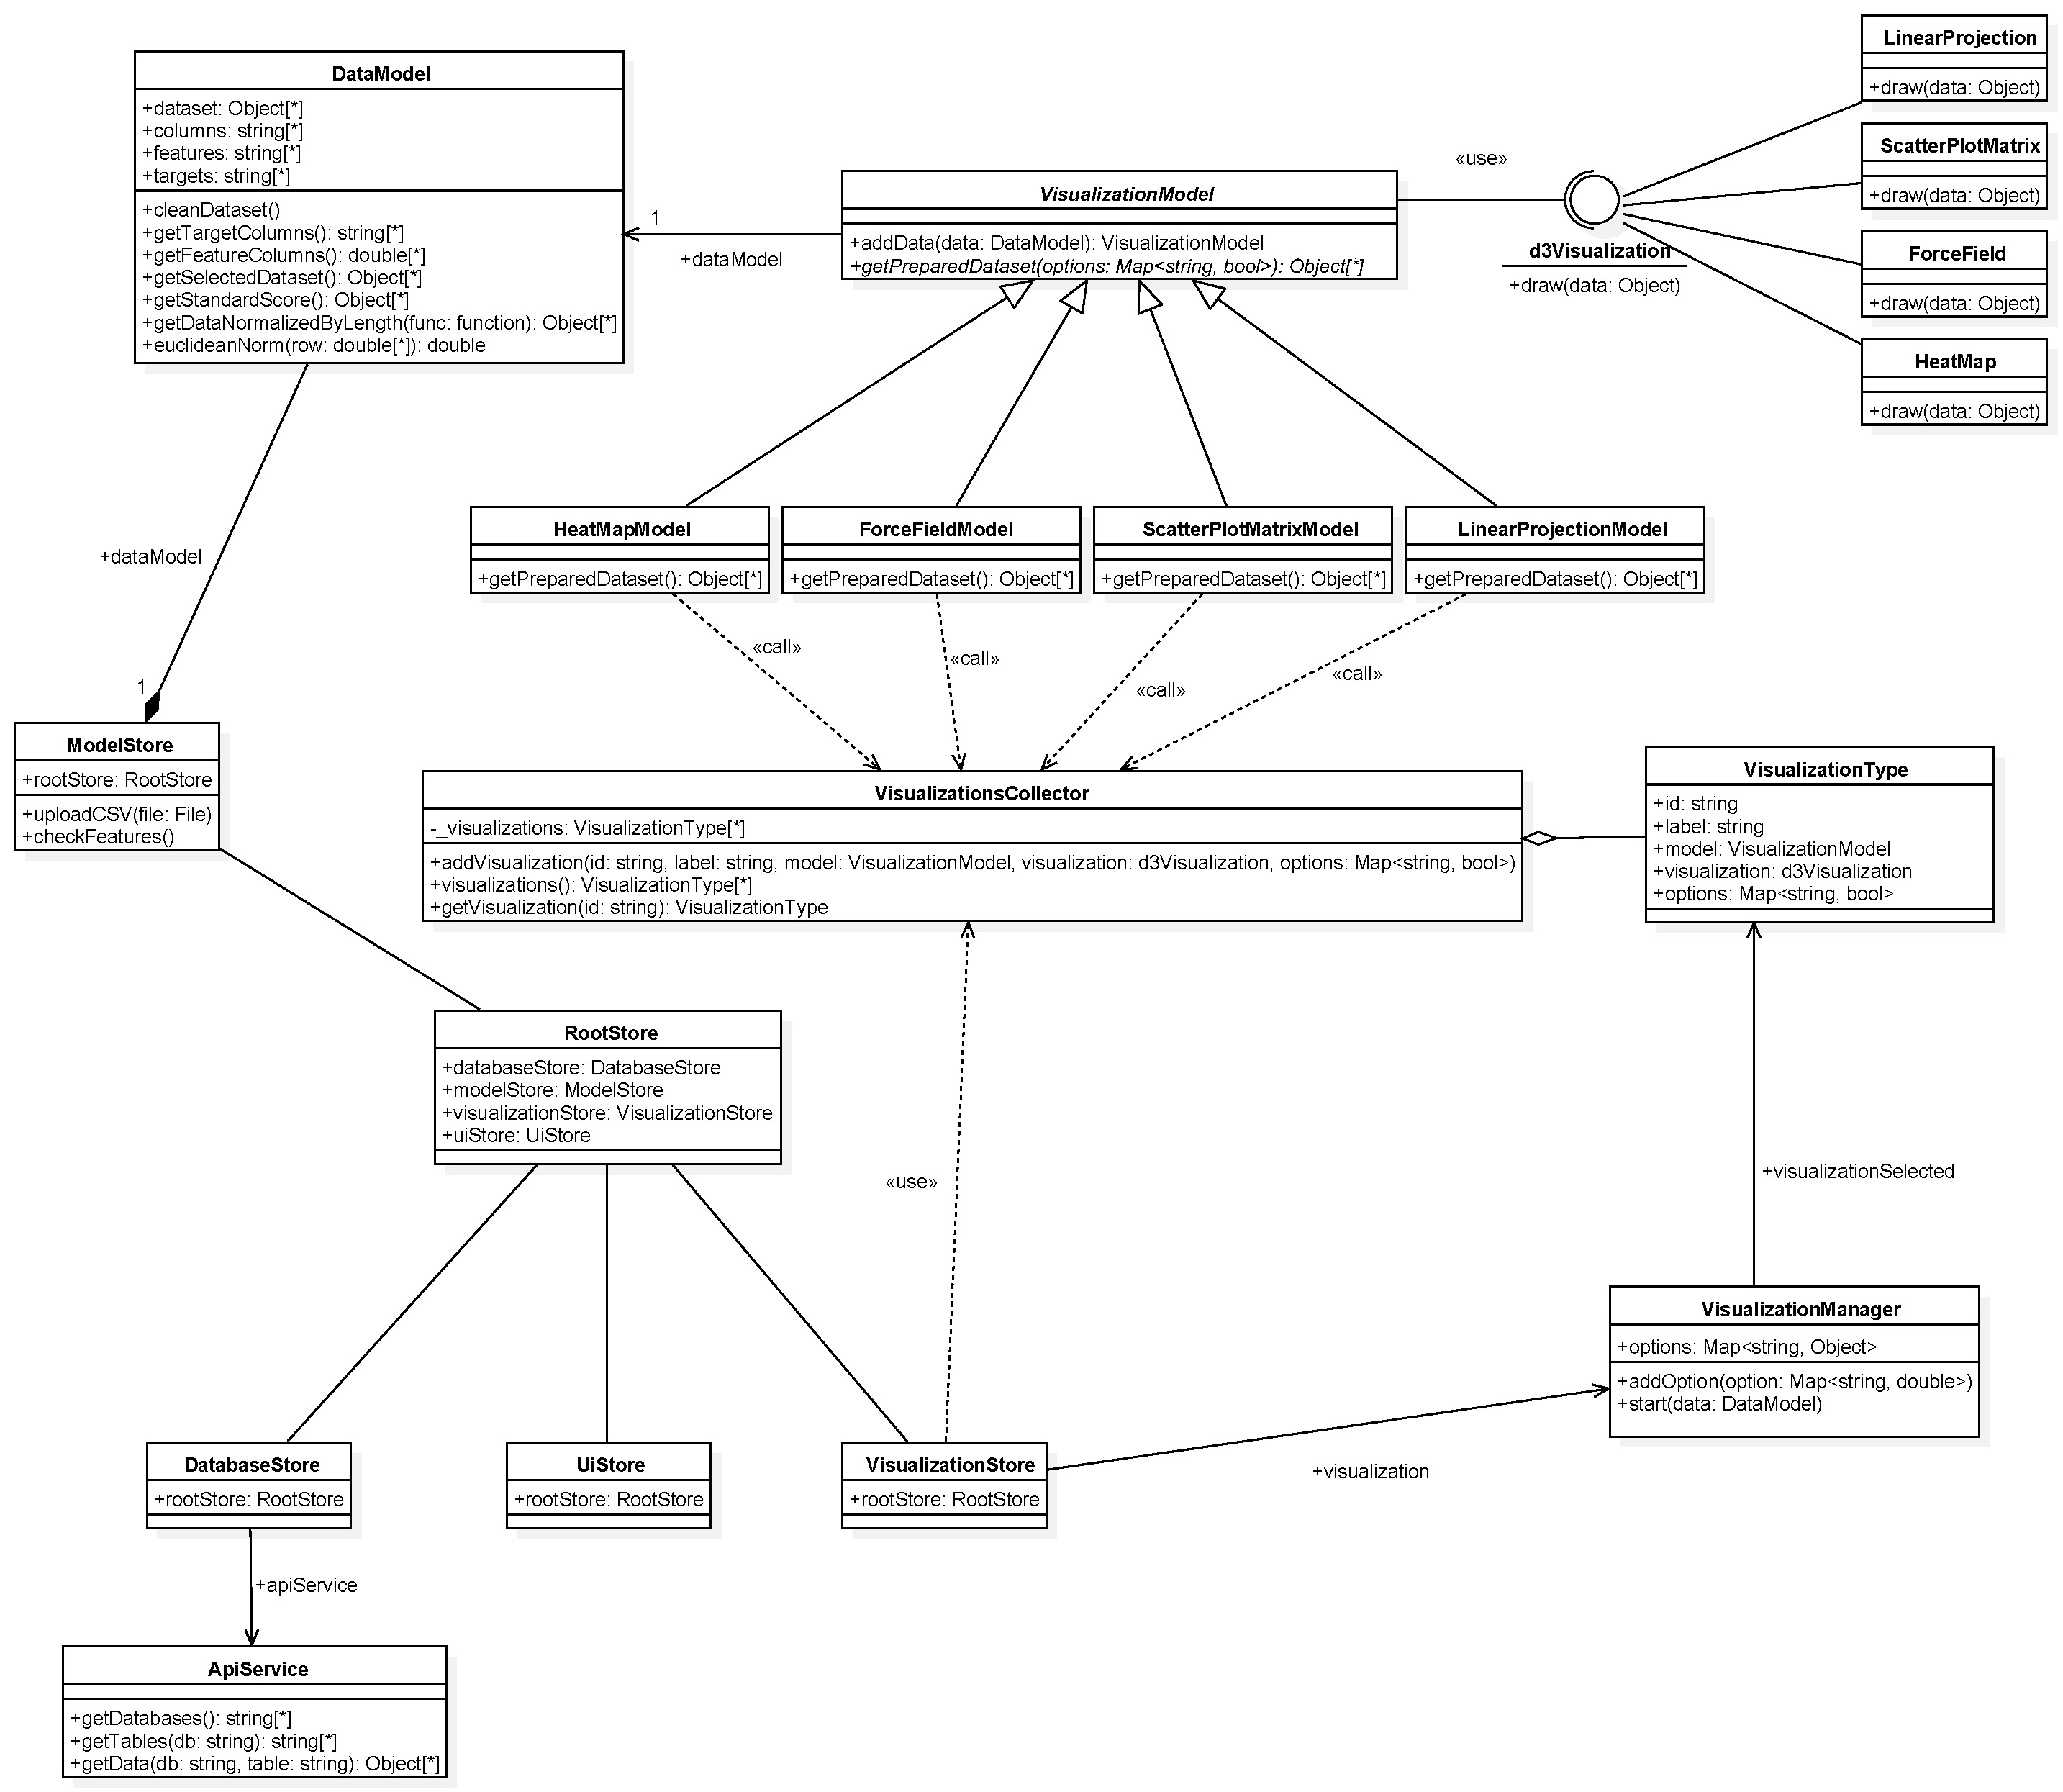
\includegraphics[width=1\textwidth]{source/img/classi.pdf}
        \caption{Diagramma delle classi della web app}
    \end{figure}
    
    \pagebreak
    
    \subsubsection{Diagrammi di sequenza}
        \paragraph{Diagramma di sequenza caricamento dati tramite CSV}
        Segue il diagramma di sequenza che modella le interazioni fra le classi coinvolte per il caricamento dei dati da file CSV.
            \begin{figure}[H]
                \centering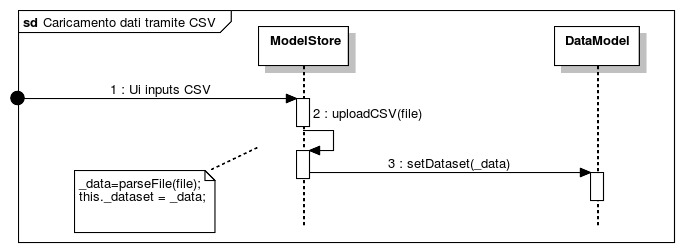
\includegraphics[width=1\textwidth]{source/img/sequenza1.jpeg}
                \caption{Diagramma di sequenza per il caricamento dati da file CSV}
            \end{figure}
            
        \paragraph{Diagramma di sequenza per la scelta del tipo di visualizzazione}
        Segue il diagramma di sequenza che modella le interazioni fra le classi coinvolte per la scelta del tipo di visualizzazione.
        \begin{figure}[H]
                \centering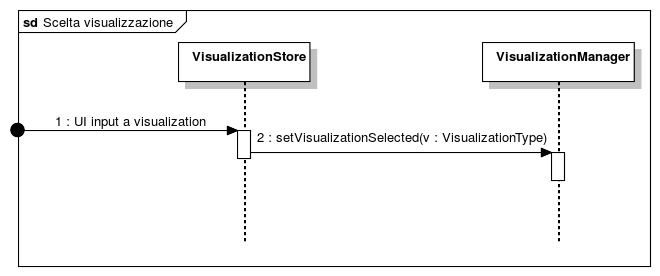
\includegraphics[width=1\textwidth]{source/img/sequenza2.jpeg}
                \caption{Diagramma di sequenza per la scelta del tipo di visualizzazione}
            \end{figure}
        \paragraph{Diagramma di sequenza per la selezione delle feature\glo\ e target}
        Segue il diagramma di sequenza che modella le interazioni fra le classi coinvolte nella selezione delle feature\glo\ e target.
        \begin{figure}[H]
                \centering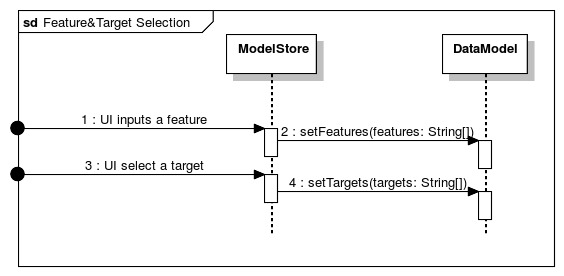
\includegraphics[width=1\textwidth]{source/img/sequenza3.jpeg}
                \caption{Diagramma di sequenza per la selezione delle feature\glo\ e target}
            \end{figure}
        
        \paragraph{Diagramma di sequenza per la selezione della distanza (opzioni generiche)}
        Segue il diagramma di sequenza che modella le interazioni fra le classi coinvolte per la selezione della distanza(e in generale di tutte le opzioni riguardanti la manipolazione del dataset).
        \begin{figure}[H]
                \centering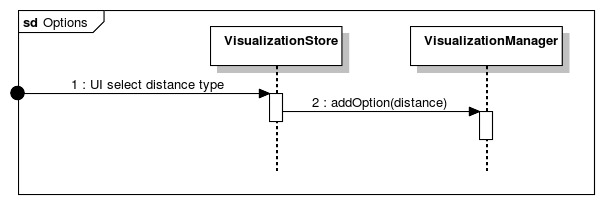
\includegraphics[width=1\textwidth]{source/img/sequenza4.jpeg}
                \caption{Diagramma di sequenza per la selezione del tipo di distanza da utilizzare per la matrice}
        \end{figure}
        
        \paragraph{Diagramma di sequenza per la visualizzazione del grafico selezionato}
        Segue il diagramma di sequenza che modella le interazioni fra le classi coinvolte per la visualizzazione del grafico scelto.
        \begin{figure}[H]
                \centering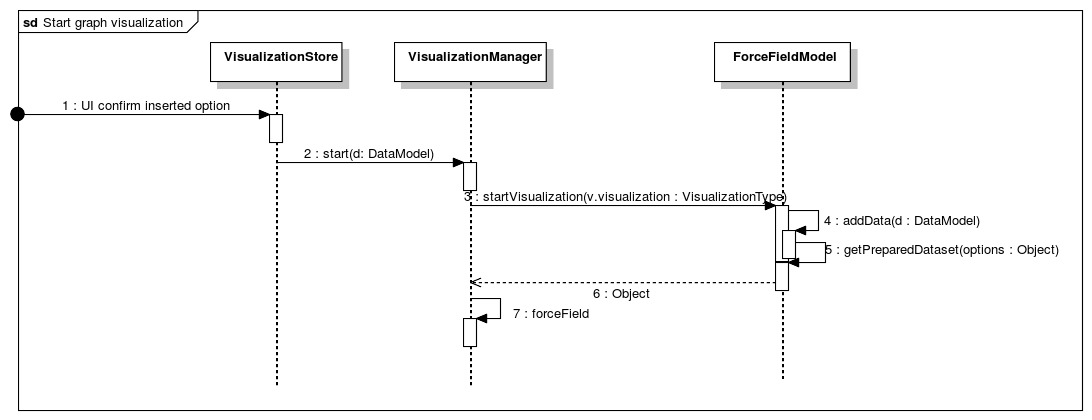
\includegraphics[width=1\textwidth]{source/img/sequenza5.jpeg}
                \caption{Diagramma di sequenza per la visualizzazione del grafico}
            \end{figure}
        
        
    \subsubsection{Design Pattern utilizzati}
        Sono stati individuati due differenti pattern, entrambi utilizzati nel model:
        \begin{itemize}
            \item Template method;
            \item Facade.
        \end{itemize}
        Per quanto riguarda il \textbf{Template method pattern}: la classe VisualizationModel è il template e i diversi tipi di visualizzazioni (ForceFieldModel, HeatMapModel,...) devono implementare VisualizationModel e in particolare il metodo \texttt{getPreparedDataset()}. La realizzazione di tale pattern, per le caratteristiche di JavaScript\glo , richiede di inserire all'interno dei metodi astratti un'eccezione, in questo modo le varie generalizzazioni sono obbligate a implementarli. L'utilizzo di questo pattern ha permesso di evitare un'espressione switch per richiamare la visualizzazione richiesta e facilita l'estensione di \hd .
        
        Allo scopo di semplificare le interazioni con il modello è stata creata una classe VisualizationManager, che funge da \textbf{Facade}. VisualizationManager fornisce una interfaccia semplificata alle componenti Store.
        
        \pagebreak
        
\subsection{Architettura server}
    \subsubsection{Descrizione}
    L'architettura server è composta da 5 moduli:
    \begin{itemize}
            \item index.js è il primo modulo eseguito e gestisce le richieste e le risposte dell'API.
            \item  controller.js ha come scopo l'indirizzamento del codice in base al tipo di database al quale ci si vuole connettere.
            \item SQL-Function.js il quale contiene le funzioni eseguite dai database di tipo SQL.
            \item Connection.js gestisce le diverse connessioni ai database.
            \item NoSQL-Function.js che contiene le funzioni per i database NoSQL.
        \end{itemize}
    Avendo la necessità di gestire connessioni a database SQL e non, abbiamo modularizzato il nostro server in modo tale da facilitare la manutenibilità e la possibilità di integrare nuove funzionalità.
    
    La gestione delle richieste API è stata possibile tramite Express. Express è un framework per applicazioni web Node.js\glo\ che fornisce molti metodi di utilità HTTP che facilita la creazione di un API.
    
    \subsubsection{Diagrammi di sequenza}
    
    \paragraph{Diagramma di sequenza per la ricerca dei nomi dei database}
     Segue il diagramma di sequenza della chiamata API getDatabases che fornisce in risposta tutti i database al quale è possibile connettersi.
            \begin{figure}[H]
                \centering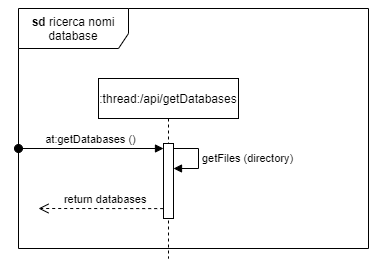
\includegraphics[width=0.6\textwidth]{source/img/API_getDatabases.png}
                \caption{Diagramma di sequenza per l'API getDatabases}
            \end{figure}
            \pagebreak

    \paragraph{Diagramma di sequenza per la ricerca dei nomi delle tabelle del database}
        Segue il diagramma di sequenza della chiamata API getTable che fornisce in risposta i metadati delle tabelle presenti ne database richiesto.
            \begin{figure}[H]
                \centering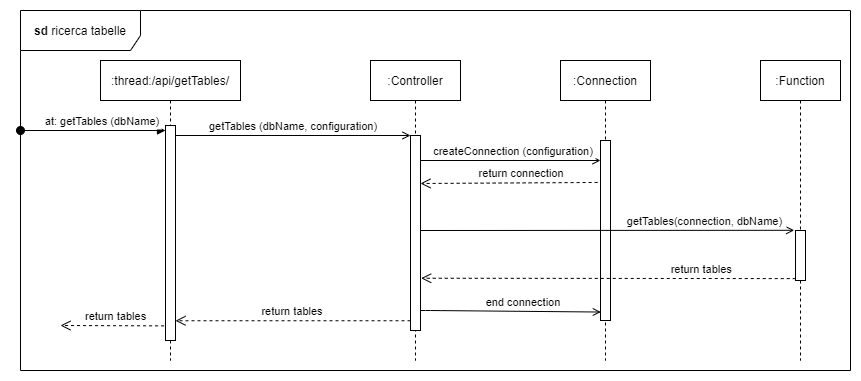
\includegraphics[width=1\textwidth]{source/img/API_getTable.png}
                \caption{Diagramma di sequenza per l'API getTable}
            \end{figure}
            
    \paragraph{Diagramma di sequenza per l'ottenimento dei dati della tabella selezionata}
    Segue il diagramma di sequenza della chiamata API getData che fornisce in risposta i metadati e dati della tabella selezionata.
            \begin{figure}[H]
                \centering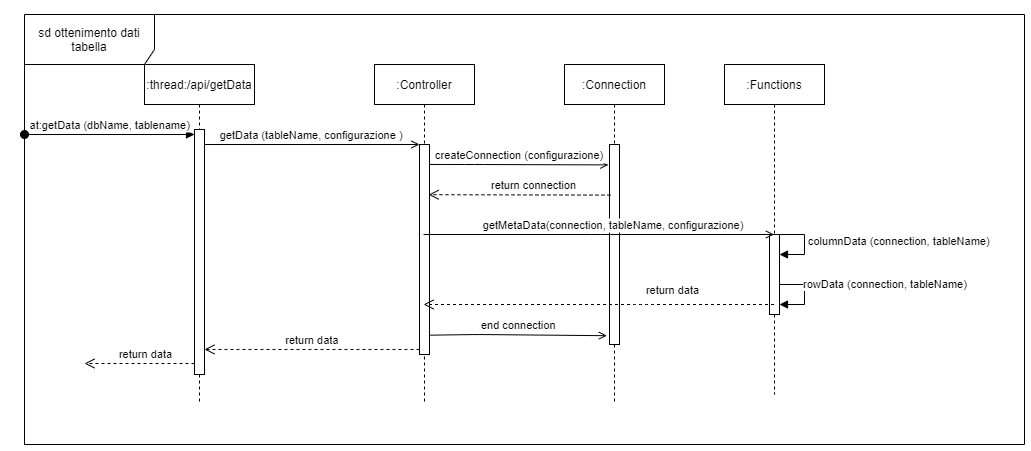
\includegraphics[width=1\textwidth]{source/img/API_getData.png}
                \caption{Diagramma di sequenza per l'API getData}
            \end{figure}
    \pagebreak
    
    \section{Estendere HD Viz}
    \subsection{Descrizione}
    \hd\ è un prodotto open source\glo\ ed in quanto tale ogni utente può modificare, estendere e ridistribuire la propria versione del codice sorgente. In questa sezione è possibile consultare le norme e le modalità attraverso le quali si può estendere e modificare il progetto \hd .
    \subsection{Contribuire al progetto principale}
    Il progetto principale è gestito dai componenti del gruppo \cod , e si può trovare al seguente repository\glo\ GitHub\glo : \href{https://github.com/CodeOfDutyJS/hdviz}{https://github.com/CodeOfDutyJS/hdviz}.
    Il gruppo \cod\ si riserva il diritto di approvare e verificare ogni modifica apportata al progetto principale.
        \subsubsection{Diagramma di attività di modifica e/o estensione al progetto}
        Il seguente diagramma illustra l'attività di modifica e/o estensione del progetto:
        \\
        \\
        \begin{figure}[H]
            \centering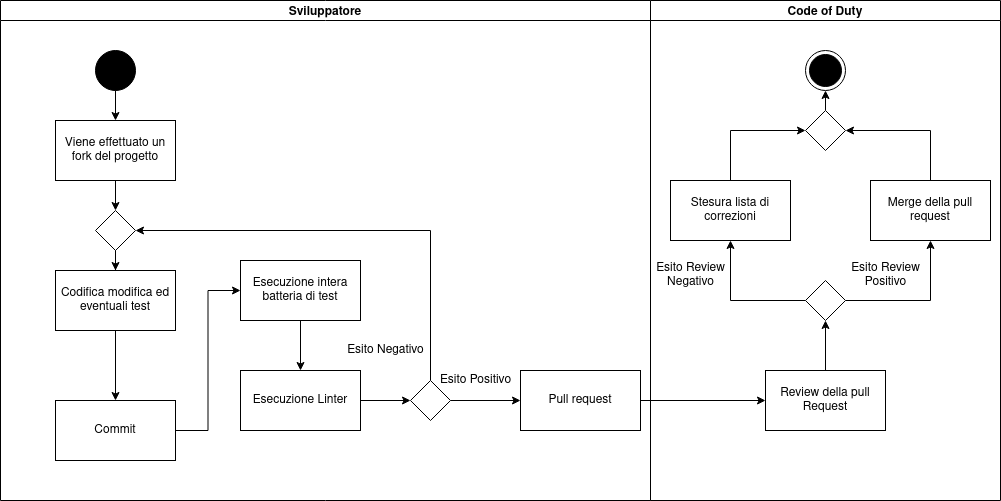
\includegraphics[width=1\textwidth]{source/img/estensione_progetto.png}
            \caption{Diagramma di sequenza per modificare/estendere \hd}
        \end{figure}
        \subsubsection{Descrizione attività di modifica e/o estensione al progetto}
        L'attività di modifica e/o estensione al progetto si svolge nel seguente modo:
        \begin{itemize}
            \item lo sviluppatore esegue un fork del progetto;
            \item codifica la modifica;
            \item codifica eventuali test necessari;
            \item esegue il commit della modifica;
            \item esegue l'intera batteria di test;
            \item esegue il linter;
            \item nel caso sia i test che il linter diano risultato positivo esegue una pull request;
            \item un membro del gruppo \cod\ esegue la review della pull request;
            \item in caso la review dia esito negativo viene stesa una lista di correzioni da eseguire;
            \item in caso la review dia esito positivo viene approvata la pull request.
        \end{itemize}
        \subsubsection{Issue}
        Alla pagina GitHub\glo\ di \hd\ è possibile trovare una board con tutte le Issue attive in un dato momento. La gestione delle Issue stesse è riservata al gruppo \cod , ma chiunque può contribuire suggerendo miglioramenti e correzioni, o segnalando eventuali bug. 
        \subsubsection{Effettuare il fork}
        Per effettuare il fork del progetto è sufficiente andare alla pagina GitHub\glo\ e cliccare sul pulsante "fork" in alto a destra.
        \subsubsection{Pull request}
        Le pull request sono soggette alle seguenti norme:
        \begin{itemize}
            \item ogni pull request deve contenere una descrizione estensiva delle modifiche e correzioni apportate al progetto, se con la pull request vengono risolte delle Issue si deve porre un riferimento alle stesse;
            \item ogni pull request è soggetta alle regole interne di \textit{Code of Duty} per quanto riguarda il processo di verifica e validazione;
            \item ogni pull request può essere commentata da qualsiasi utente;
            \item il gruppo \textit{Code of Duty} si riserva il diritto ultimo di approvare o chiudere una pull request, in ogni caso una modifica allo stato della pull request deve essere giustificata con un commento;
            \item il gruppo \textit{Code of Duty} non assicura alcun limite di tempo al processo di review.
        \end{itemize}
        \subsubsection{Stesura dei test}
        La stesura dei test viene riconosciuta dal gruppo \textit{Code of Duty} come buona pratica per la stesura di codice di qualità. Chiunque voglia contribuire scrivendo test per l'applicazione o per testare la propria estensione e/o modifica del codice deve:
        \begin{itemize}
            \item usare il framework Jest
            \item seguire le convenzioni del gruppo sul nome dei file di test, cioè usare la seguente convenzione per i nomi dei file:
            \begin{verbatim}
                nomeClasse.spec.js
            \end{verbatim}
            dove nomeClasse è il nome della classe da testare;
            \item porre i file di test nella cartella corrispondente nell'albero di test, ad esempio se si vuole testare
            \begin{verbatim}
                hdviz/client/src/d3/newVisualization.js
            \end{verbatim}
            inserire il test in:
            \begin{verbatim}
                hdviz/client/src/test/d3/newVisualization.spec.js
            \end{verbatim}.
        \end{itemize}
    \subsection{Usare HD Viz come base per un altro progetto}
    \hd\ è un progetto open source\glo , chiunque può usare il codice del progetto in parte o nella sua interezza e ridistribuirlo gratuitamente o dietro pagamento.
    \subsection{Aggiungere una visualizzazione}
    Per aggiungere una visualizzazione creare un nuovo file .js in:
    \begin{verbatim}
        client/src/model/d3
    \end{verbatim}
    all'interno del file creare una funzione contenente il codice d3 da eseguire. Per convenzione d3 all'interno del progetto viene importato con:
    \begin{verbatim}
        import * as d3 from 'd3';
    \end{verbatim}
    \hd\ contiene un unico elemento svg con id \#area, questo è utile per la manipolazione del DOM in quanto rende il svg selezionabile con un sola istruzione d3:
    \begin{verbatim}
        const svg = d3.select('#area');
    \end{verbatim}
        \subsubsection{Inserire la nuova visualizzazione}
        Ogni visualizzazione deve essere associata ad un modello. Ogni modello implementa la funzione  \texttt{getPreparedDataset()}, che ritorna i dati alla visualizzazione. Se si vuole sfruttare un modello già esistente è necessario creare una nuova classe che eredita dal modello e implementare nuovamente \texttt{getPreparedDataset()} con i dati necessari alla propria visualizzazione. Successivamente perché la visualizzazione sia disponibile e selezionabile dalla UI è sufficiente aggiungere un \texttt{VisualizationType} nel \texttt{VisualizationCollector}, in questo modo:
        \begin{verbatim}
            VisualizationCollector.addVisualization({
              id: 'myviz',
              label: 'My Visualization',
              model: new MyVisualizationModel(),
              visualization: myVisualization,
              options: { distance: true },
            });
        \end{verbatim}
        
        Per convenzione questa porzione di codice viene inserita all'interno del file del suo corrispondente \texttt{VisualizationModel}, fuori dallo scope della classe.
        
        I parametri che vengono passati a \texttt{.addVisualization()} sono:
        \begin{itemize}
            \item \textbf{id}: id univoco per la visualizzazione;
            \item \textbf{label}: testo che viene mostrato nella UI per la selezione della visualizzazione;
            \item \textbf{model}: l'oggetto del nuovo modello di visualizzazione;
            \item \textbf{visualization}: la funzione della nuova visualizzazione;
            \item \textbf{options}: le opzioni che la UI deve visualizzare, nell'esempio distance, quindi verrà visualizzata la selezione del tipo di distanza.
        \end{itemize}
    
        Una volta aggiunta la visualizzazione al \texttt{VisualizationCollector} è necessario importare il nuovo file all'interno del file index.js nella cartella VisualizationModels.
        
        \subsubsection{Pratiche usate dal gruppo usando d3}
            Questa sezione contiene pratiche che pur non essendo convenzionate sono considerate dal gruppo utili per la creazione di visualizzazioni d3.
            \myparagraph{Utilizzo di tag g}
            Pur non essendo strettamente necessario creare dei gruppi all'interno dei quali inserire (o come lo definisce d3 "appendere") gli elementi sui quali andrà effettivamente eseguito il data binding si rivela molto utile a livello organizzativo e gestionale, in particolare le operazioni di trasformazioni applicate all'intero gruppo si riflettono su tutti i suoi membri, mentre quelle all'interno del gruppo sono relative alla trasformazione "padre".
            \myparagraph{Resize e dimensioni dell'svg}
            Il resize dello schermo può essere gestito molto semplicemente in particolare il modo per inserire una callback all'evento onresize è il seguente:
            \begin{verbatim}
            d3.select('window')
              .on('resize', callback);
            \end{verbatim}
            dove l'utente può inserire una qualsiasi funzione al posto di callback. Viene da se che per gestire l'evento di resize si dovrà disegnare di nuovo la visualizzazione. Quindi si rende necessario "pulire" lo schermo con:
            \begin{verbatim}
                d3.select('#area').selectAll('*').remove();
            \end{verbatim}
            e poi successivamente a richiamare la propria funzione di visualizzazione.
            Si rende però altresì necessario esprimere le dimensioni della visualizzazione rispetto alle dimensioni del svg. Queste possono essere trovate con:
            \begin{verbatim}
                const { width, height } = svg.node().getBoundingClientRect();
            \end{verbatim}
    \subsection{Aggiungere un modello}
    Le classi modello vengono aggiunte all'interno di:
    \begin{verbatim}
        client/src/model/VisualizationModels
    \end{verbatim}
    solitamente la classe di modello viene chiamata come la funzione di visualizzazione con l'aggiunta di Model, ad esempio:
    \begin{verbatim}
        LinearProjection
    \end{verbatim}
    diventa:
    \begin{verbatim}
        LinearProjectionModel
    \end{verbatim}
    Si deve ereditare da \texttt{VisualizationModel}. Si deve implementare il metodo \texttt{getPreparedDataset()}, restituendo un oggetto contenente i dati da passare alla funzione di visualizzazione.
    
    Il metodo \texttt{getPreparedDataset()} per convenzione può avere in input delle opzioni, come la funzione di distanza o di normalizzazione da utilizzare.
    
    se si vuole ricevere in input queste opzioni è necessario riceverle come oggetto:
    
    \begin{verbatim}
        getPreparedDataset({ distanceFn, normalizeFn }){
            ...
        }
    \end{verbatim}
    Per convenzione se si vuole richiedere la funzione di distanza è necessario aggiungere \texttt{distanceFn} mentre per la funzione di normalizzazione è necessario aggiungere \texttt{normalizeFn}.
    
    \subsection{Aggiungere una legenda}
    Vengono fornite due funzioni, dentro \texttt{client/src/model/d3}
    chiamate \texttt{drawTargetLegend()} e \texttt{drawColorScale()}.
    \texttt{drawTargetLegend()} si occupa di disegnare la leggenda dei target, assegna colore e testo ad ogni valore differente di target, ed ha la seguente firma:
    \begin{verbatim}
        function drawTargetLegend(color, target, x, y, height, width) 
    \end{verbatim}
    dove:
    \begin{itemize}
        \item \texttt{color} è la funzione di colore d3 usata per assegnare i colori ai target, basta passare la stessa funzione usata nella funzione di visualizzazione;
        \item \texttt{target} è un array contenente gli oggetti target, si può passare direttamente\\\texttt{this.dataModel.getTargetColumns()} dal modello;
        \item \texttt{x} è la coordinata x della legenda;
        \item \texttt{y} è la coordinata y della legenda;
        \item \texttt{height} è l'altezza della legenda;
        \item \texttt{width} è la larghezza della legenda.
    \end{itemize}
    mentre \texttt{drawColorScale()} ha la seguente firma:
    \begin{verbatim}
        function drawColorScale(color, range, x, y, width, height, name)
    \end{verbatim}
    e si occupa di disegnare un range di colori con la scala associata. i parametri sono gli stessi ad eccezione di:
    \begin{itemize}
        \item \texttt{range}: un array nella forma [min, max] dove min e max sono gli estremi del range di visualizzazione, alternativamente è possibile passare un array contenente tutti i valori della visualizzazione;
        \item \texttt{name}: una stringa rappresentante il nome della scala.
    \end{itemize}
    
    \appendix
    \section{Glossario}
    \subsection{API Rest}
    Acronimo per Application Programming Interface. Sono un insieme di definizioni e protocolli
    per l’integrazione di software. REST è un insieme di principi architetturali per sviluppare API.

    \subsection{Backend}
    Parte di una soluzione software che gestisce elabora e utilizza i dati forniti dal frontend.

    \subsection{d3.js}
    Libreria JavaScript per creare visualizzazioni sul web.

    \subsection{Feature}
    Campo dati solitamente numerico che fornisce un’informazione su una caratteristica. (es: Lunghezza Altezza)

    \subsection{Frontend}
    Parte di una soluzione software che interagisce con l’utente.

    \subsection{GitHub}
    Piattaforma per versionamento tramite Git e condivisione di codice. Fornisce anche strumenti
    di CI/CD.

    \subsection{JavaScript}
    Linguaggio di programmazione orientato agli oggetti e agli eventi.

    \subsection{Node.js}
    Runtime orientato agli eventi asincroni per l’esecuzione di codice JavaScript.

    \subsection{Open source}
    Termine per indicare un tipo di software che tramite una licenza i detentori dei diritti favoriscono
    la modifica lo studio l’utilizzo e la redistribuzione del codice sorgente.

    \subsection{React}
    Libreria JavaScript per la creazione di interfacce utente.

    \subsection{Repository}
    Ambiente in cui vengono conservati e gestiti i file di un progetto.

    
\end{document}